\chapter{TINJAUAN PUSTAKA}

\section{Landasan Teori}

\subsection{Traffic Engineering}
\textit{Traffic Engineering} (TE) adalah disiplin rekayasa jaringan yang berfokus pada pengukuran, pemodelan, karakterisasi, dan kontrol lalu lintas internet untuk mengoptimalkan kinerja jaringan. Tujuan utama TE adalah meminimalkan kongesti dan meningkatkan pemanfaatan sumber daya melalui penyeimbangan beban trafik (\textit{load balancing}) \cite{marouani2024}.

TE modern membutuhkan kemampuan untuk menangani pola trafik yang dinamis dan beragam, di mana pendekatan konvensional berbasis algoritma statis seperti jalur terpendek (Dijkstra) seringkali tidak mampu beradaptasi dengan kondisi jaringan yang berubah secara real-time. Oleh karena itu, pendekatan berbasis kecerdasan buatan semakin diperlukan untuk melakukan optimasi distribusi trafik secara adaptif dan efisien.

\begin{figure}[H]
    \centering
    \includegraphics[width=0.8\textwidth]{images/te.png}
    \caption{Ilustrasi Traffic Engineering dalam Jaringan}
    \label{fig:traffic_engineering}
\end{figure}

\subsection{Jaringan Layer 2 dan VLAN}
Jaringan Layer 2 beroperasi pada lapisan \textit{Data Link} dalam model OSI, di mana perangkat \textit{switch} mengirimkan frame berdasarkan alamat MAC\@. Teknologi VLAN (\textit{Virtual Local Area Network}) memungkinkan segmentasi jaringan secara logis dalam satu infrastruktur fisik, meningkatkan keamanan dan efisiensi manajemen jaringan. Segmentasi VLAN terbukti dapat meningkatkan performa jaringan dengan membagi \textit{broadcast domain} yang besar menjadi domain-domain yang lebih kecil dan terkelola \cite{warse2025vlan}.

Pada lingkungan ISP yang menggunakan infrastruktur \textit{switching} Layer 2 dengan VLAN, penerapan Traffic Engineering menghadapi tantangan khusus. Mekanisme \textit{Spanning Tree Protocol} (STP) pada Layer 2 cenderung memblokir jalur redundan untuk mencegah \textit{looping}, yang mengakibatkan tautan cadangan tidak termanfaatkan (\textit{underutilized}) \cite{rashid2024performance, aruba2025campus}. Meskipun varian yang lebih modern seperti \textit{Rapid Spanning Tree Protocol} (RSTP) menawarkan konvergensi yang lebih cepat, kondisi ini tetap membuat optimasi jalur menjadi lebih kompleks dibandingkan jaringan IP tradisional (Layer 3) \cite{ahmad2020intervlan}. Oleh karena itu, diperlukan pendekatan cerdas untuk memprediksi kegagalan dan mendistribusikan trafik secara dinamis tanpa melanggar topologi logis Layer 2 \cite{alhachem2025}.

\begin{figure}[H]
    \centering
    % \includegraphics[width=0.8\textwidth]{images/layer2_vlan.png}
    \caption{Arsitektur Jaringan Layer 2 dengan VLAN}
    \label{fig:layer2_vlan}
\end{figure}

\subsection{Kriteria Evaluasi Kualitas Jalur}

Dalam penelitian ini, kualitas jalur jaringan dievaluasi berdasarkan dua kategori utama kriteria: kriteria tingkat node dan kriteria tingkat edge. Pendekatan dual-level ini memastikan evaluasi yang komprehensif dengan mempertimbangkan baik kemampuan perangkat maupun kualitas koneksi \cite{joint_node_edge_optimization, holistic_network_metrics}.

\subsubsection{Kriteria Tingkat Node}

Kriteria tingkat node mengevaluasi kapasitas dan kondisi operasional dari perangkat jaringan (switch/router) yang dilalui oleh sebuah jalur. Berdasarkan literatur resource-aware routing \cite{resource_aware_sdn, node_capacity_routing}, kriteria yang dipilih adalah:

\begin{enumerate}
    \item \textbf{CPU Score}: Normalized CPU utilization yang menunjukkan ketersediaan processing power. CPU utilization merupakan indikator krusial untuk memastikan node tidak overloaded, yang dapat menyebabkan packet processing delay \cite{cpu_aware_routing, resource_aware_sdn}.

    \item \textbf{RAM Score}: Normalized memory availability untuk buffering dan state management. Ketersediaan memori mempengaruhi kemampuan buffering dan handling concurrent connections \cite{resource_aware_sdn, node_capacity_routing}.

    \item \textbf{Traffic Score}: Volume trafik yang sedang ditangani node. Current traffic load merupakan metric penting untuk load balancing dan congestion avoidance \cite{utilization_based_te, adaptive_utilization_routing}.

    \item \textbf{Utilization Score}: Aggregate interface utilization yang menunjukkan seberapa sibuk node dalam menangani trafik \cite{interface_speed_impact, utilization_based_te}.

    \item \textbf{Status Score}: Binary indicator operational status (up/down) yang sangat penting untuk failure-aware routing \cite{failure_aware_te}.
\end{enumerate}

Skor komposit node dihitung sebagai weighted sum:
\begin{equation}
    S_{node} = \sum_{i=1}^{5} w_i^{node} \cdot f_i^{node}
\end{equation}

\noindent dimana $w_i^{node}$ adalah bobot kriteria yang diperoleh dari AHP dan $f_i^{node}$ adalah nilai kriteria yang telah dinormalisasi. Pemilihan kriteria node ini mengikuti pendekatan resource-aware routing yang mempertimbangkan kapasitas processing dan forwarding capability dari setiap perangkat jaringan \cite{joint_node_edge_optimization, holistic_network_metrics}.

\subsubsection{Kriteria Tingkat Edge}

Kriteria tingkat edge mengevaluasi karakteristik koneksi fisik atau logis antar perangkat. Mengikuti framework multi-constraint routing \cite{te_multiconstraint, sdn_multiconstraint_routing}, kriteria yang dipilih meliputi:

\begin{enumerate}
    \item \textbf{Optical Link Quality Score}: Kualitas sinyal optik berdasarkan Optical Signal-to-Noise Ratio (OSNR), received power, Q-factor, atau chromatic dispersion pada fiber optic infrastructure \cite{optical_signal_quality, fiber_link_quality, osnr_monitoring}. Semakin tinggi kualitas sinyal optik, semakin reliable physical layer transmission.

    \item \textbf{Error Rate Score}: Inverse dari Bit Error Rate (BER) atau Packet Error Rate (PER) yang menunjukkan reliabilitas data transmission \cite{ber_per_optical, ber_monitoring, error_rate_impact}. Metrik ini berbeda dari optical quality karena mengukur actual transmission errors setelah decoding.

    \item \textbf{Packet Loss Score}: Inverse dari packet loss rate untuk mengindikasikan reliability. Persentase paket yang hilang atau dropped selama transmisi, yang dapat disebabkan oleh congestion, buffer overflow, atau TTL expiry \cite{packet_loss_detection}.

    \item \textbf{Bandwidth Utilization (a→b, b→a)}: Utilisasi bandwidth pada kedua arah link merupakan indikator critical untuk menghindari congestion \cite{bandwidth_aware_te, utilization_based_te}.

    \item \textbf{Interface Speed (a, b)}: Maximum capacity kedua endpoint yang menentukan throughput ceiling dari link \cite{interface_speed_impact, qos_composite_metric}.

    \item \textbf{Distance}: Geographic atau logical distance yang mempengaruhi propagation delay dan dapat menjadi faktor dalam path cost calculation \cite{geographic_routing, distance_aware_datacenter, latency_distance_routing}.

    \item \textbf{Status}: Link operational state (up/down) essential untuk topology-aware routing \cite{link_state_routing, failure_aware_te}.
\end{enumerate}

Skor komposit edge dihitung sebagai:
\begin{equation}
    S_{edge} = \sum_{j=1}^{9} w_j^{edge} \cdot g_j^{edge}
\end{equation}

\noindent dimana kini terdapat 9 kriteria edge. Pemisahan antara optical signal quality, error rate, dan packet loss penting karena ketiganya mengukur aspek yang berbeda dari reliability link pada layer yang berbeda.

\paragraph{Perbedaan Optical Quality, Error Rate, dan Packet Loss}

Ketiga metrik ini saling melengkapi dalam mengevaluasi kualitas koneksi pada layer yang berbeda:

\begin{enumerate}
    \item \textbf{Optical Link Quality} (Physical Layer): Mengukur kualitas sinyal cahaya pada fiber optic sebelum proses decoding. Parameter seperti OSNR (Optical Signal-to-Noise Ratio), received optical power (dBm), Q-factor, dan chromatic dispersion mengindikasikan seberapa baik sinyal optik dapat dibedakan dari noise \cite{optical_signal_quality, osnr_monitoring}. Degradasi optical quality dapat disebabkan oleh attenuasi fiber, dispersion, atau interferensi optik.

    \item \textbf{Error Rate} (Data Link Layer): Mengukur tingkat kesalahan bit atau paket setelah proses photodetection, analog-to-digital conversion, dan forward error correction (FEC). BER atau PER menunjukkan berapa banyak bit/paket yang corrupt setelah decoding \cite{ber_per_optical, ber_monitoring}. Bahkan dengan optical quality yang baik, error rate bisa tinggi jika ada masalah pada transceiver atau proses decoding.

    \item \textbf{Packet Loss Rate} (Network Layer): Mengukur paket yang hilang atau di-drop karena congestion, buffer overflow, atau TTL expiry, bukan karena corruption \cite{packet_loss_detection}. Packet loss dapat terjadi meskipun optical quality baik dan error rate rendah, terutama saat terjadi congestion pada switch/router.
\end{enumerate}

Kombinasi ketiga metrik ini memberikan gambaran holistik tentang health dari sebuah link, dari physical layer hingga network layer \cite{holistic_network_metrics}. Integrasi multiple edge metrics ini mengikuti paradigma multi-criteria path selection yang telah terbukti efektif dalam traffic engineering modern \cite{routing_multiple_optimality, madm_heuristic_routing, te_multiconstraint, sdn_multiconstraint_routing}.

Pendekatan weighted composite scoring yang mengintegrasikan kriteria node dan edge ini telah terbukti efektif dalam various QoS routing scenarios \cite{qos_composite_metric, weighted_composite_routing, madm_heuristic_routing, routing_multiple_optimality}.

\subsection{Graph Attention Network (GAT)}

\textit{Graph Attention Network} (GAT) merupakan pengembangan lanjut dari \textit{Graph Neural Networks} (GNN) yang memperkenalkan mekanisme \textit{masked self-attention} untuk mengatasi keterbatasan metode berbasis graf konvensional. Berbeda dengan GNN tradisional yang memperlakukan semua tetangga node dengan bobot yang sama atau bergantung pada struktur graf yang telah ditentukan sebelumnya, GAT memiliki kemampuan untuk secara adaptif menentukan tingkat kepentingan (\textit{attention coefficients}) dari setiap node tetangga \cite{velickovic2017}.

Dalam konteks jaringan komputer, mekanisme atensi ini sangat relevan karena tidak semua jalur yang terhubung memiliki kualitas yang setara. Sebagai contoh, dalam topologi jaringan PT Lare Osing Ndo, sebuah switch mungkin memiliki beberapa jalur alternatif menuju switch tujuan, namun kualitas masing-masing jalur dapat berbeda secara signifikan bergantung pada kondisi beban trafik, kapasitas bandwidth, dan performa perangkat. GAT memungkinkan model untuk "memperhatikan" jalur dengan kualitas sinyal lebih baik dan secara otomatis mengabaikan atau memberikan bobot rendah pada jalur yang mengalami degradasi \cite{kato2024}.

\subsubsection{Representasi Graf Jaringan}

Sebelum memahami mekanisme GAT, perlu dipahami terlebih dahulu bagaimana topologi jaringan direpresentasikan sebagai graf matematis. Sebuah jaringan komputer dapat dimodelkan sebagai graf tidak berarah $\mathcal{G} = (\mathcal{V}, \mathcal{E})$, dimana:

\begin{itemize}
    \item $\mathcal{V} = \{v_1, v_2, \ldots, v_N\}$ adalah himpunan node yang merepresentasikan perangkat jaringan (switch, router, atau endpoint)
    \item $\mathcal{E} \subseteq \mathcal{V} \times \mathcal{V}$ adalah himpunan edge yang merepresentasikan koneksi fisik atau logis antar perangkat
    \item $N = |\mathcal{V}|$ adalah jumlah total node dalam jaringan
    \item $M = |\mathcal{E}|$ adalah jumlah total edge (koneksi) dalam jaringan
\end{itemize}

\paragraph{Fitur Node}
Setiap node memiliki vektor fitur input yang dapat dinyatakan sebagai:

\begin{equation}
    \vec{h}_i \in \mathbb{R}^F
\end{equation}

\noindent dimana $F$ adalah dimensi fitur. Dalam kasus jaringan PT Lare Osing Ndo, fitur node dapat mencakup:

\begin{itemize}
    \item \textbf{Utilisasi CPU (\%)}: CPU utilization merupakan indikator krusial untuk memastikan node tidak overloaded, yang dapat menyebabkan packet processing delay \cite{cpu_aware_routing, resource_aware_sdn}.

    \item \textbf{Konsumsi memori RAM (\%)}: Ketersediaan memori mempengaruhi kemampuan buffering dan handling concurrent connections \cite{resource_aware_sdn, node_capacity_routing}.

    \item \textbf{Volume trafik saat ini (Mbps)}: Current traffic load merupakan metric penting untuk load balancing dan congestion avoidance \cite{utilization_based_te, adaptive_utilization_routing}.

    \item \textbf{Utilisasi interface}: Aggregate interface utilization menunjukkan seberapa sibuk node dalam menangani trafik \cite{interface_speed_impact}.

    \item \textbf{Status node}: Operational status (up/down) sangat penting untuk failure-aware routing \cite{failure_aware_te}.
\end{itemize}

Pemilihan kriteria node ini mengikuti pendekatan resource-aware routing yang mempertimbangkan kapasitas processing dan forwarding capability dari setiap perangkat jaringan \cite{joint_node_edge_optimization, holistic_network_metrics}.

\paragraph{Fitur Edge}
Selain fitur pada node, setiap edge yang menghubungkan dua node juga memiliki atribut yang merepresentasikan karakteristik koneksi tersebut. Fitur edge dapat direpresentasikan sebagai:

\begin{equation}
    e_{ij} = (v_i, v_j) \in \mathcal{E}
\end{equation}

\begin{equation}
    \vec{e}_{ij} \in \mathbb{R}^{F_e}
\end{equation}

\noindent dimana $F_e$ adalah dimensi fitur edge. Fitur-fitur ini meliputi:

\begin{itemize}
    \item \textbf{Optical Link Quality}: Kualitas sinyal optik yang diukur melalui parameter seperti Optical Signal-to-Noise Ratio (OSNR), received optical power (dBm), Q-factor, atau chromatic dispersion pada fiber optic links \cite{optical_signal_quality, fiber_link_quality, osnr_monitoring}. Metrik ini mengukur kualitas fisik sinyal optik pada physical layer sebelum terjadi decoding.

    \item \textbf{Error Rate}: Bit Error Rate (BER) atau Packet Error Rate (PER) yang mengindikasikan tingkat kesalahan transmisi data setelah proses decoding \cite{ber_per_optical, error_rate_impact, ber_monitoring}. Parameter ini mengukur reliabilitas actual data transmission pada data link layer dan berbeda dari optical signal quality karena mencerminkan end-to-end transmission reliability setelah forward error correction.

    \item \textbf{Packet Loss Rate}: Persentase paket yang hilang atau dropped selama transmisi, yang dapat disebabkan oleh congestion, buffer overflow, atau TTL expiry pada network layer \cite{packet_loss_detection}. Metrik ini melengkapi error rate dengan menangkap packet-level failures yang bukan disebabkan oleh corruption.

    \item \textbf{Bandwidth Utilization (bidirectional)}: Utilisasi bandwidth pada kedua arah link (a→b dan b→a) merupakan indikator critical untuk menghindari congestion \cite{bandwidth_aware_te, utilization_based_te}.

    \item \textbf{Interface Speed (kedua endpoint)}: Kapasitas maksimum interface pada kedua endpoint menentukan throughput ceiling dari link \cite{interface_speed_impact, qos_composite_metric}.

    \item \textbf{Geographic Distance}: Jarak fisik mempengaruhi propagation delay dan dapat menjadi faktor dalam path cost calculation \cite{geographic_routing, distance_aware_datacenter, latency_distance_routing}.

    \item \textbf{Link Status}: Operational state (up/down) essential untuk topology-aware routing \cite{link_state_routing, failure_aware_te}.
\end{itemize}

Integrasi multiple edge metrics ini mengikuti paradigma multi-criteria path selection yang telah terbukti efektif dalam traffic engineering modern \cite{routing_multiple_optimality, madm_heuristic_routing, te_multiconstraint, sdn_multiconstraint_routing}.

\paragraph{Matriks Adjacency}
Struktur konektivitas graf dapat direpresentasikan menggunakan matriks adjacency:

\begin{equation}
    \mathbf{A} \in \{0,1\}^{N \times N}
\end{equation}

\noindent dimana:

\begin{equation}
    A_{ij} = \begin{cases}
        1 & \text{jika } (v_i, v_j) \in \mathcal{E} \\
        0 & \text{jika sebaliknya}
    \end{cases}
\end{equation}

Untuk graf tidak berarah (seperti topologi jaringan Layer 2), matriks adjacency bersifat simetris. Matriks ini menjadi dasar dalam menentukan himpunan tetangga yang dapat dinyatakan sebagai:

\begin{equation}
    \mathcal{N}_i = \{v_j : A_{ij} = 1\}
\end{equation}

\noindent yang akan digunakan dalam komputasi atensi GAT.

\paragraph{Representasi Edge dalam GAT}
Dalam implementasi GAT standar, fitur edge tidak secara eksplisit dimasukkan ke dalam perhitungan koefisien atensi. Namun, untuk aplikasi Traffic Engineering, fitur edge sangat penting karena kualitas link menjadi faktor krusial dalam penentuan jalur. Oleh karena itu, terdapat beberapa strategi untuk mengintegrasikan fitur edge:

\begin{enumerate}
    \item \textbf{Edge Feature Concatenation}: Fitur edge digabungkan dengan fitur node dalam perhitungan skor atensi:
    \begin{equation}
        e_{ij} = \text{LeakyReLU}\left(\vec{a}^T [W\vec{h}_i \, \| \, W\vec{h}_j \, \| \, W_e\vec{e}_{ij}]\right)
    \end{equation}
    \noindent dimana $W_e$ adalah matriks bobot untuk transformasi fitur edge.

    \item \textbf{Edge Gating}: Fitur edge digunakan sebagai gating mechanism untuk memodulasi koefisien atensi:
    \begin{equation}
        \alpha_{ij}^{gated} = \alpha_{ij} \cdot \sigma(W_g \vec{e}_{ij})
    \end{equation}
    \noindent dimana $\sigma$ adalah fungsi sigmoid dan $W_g$ adalah matriks bobot gating.

    \item \textbf{Pre-aggregation Weighting}: Fitur edge digunakan untuk memberikan bobot awal sebelum mekanisme atensi:
    \begin{equation}
        \tilde{\alpha}_{ij} = w_{ij} \cdot \alpha_{ij}
    \end{equation}
    \noindent dimana $w_{ij}$ adalah bobot yang diturunkan dari fitur edge (misalnya, bandwidth yang tersedia atau inverse dari error rate).
\end{enumerate}

Pemilihan strategi integrasi fitur edge bergantung pada kompleksitas model yang diinginkan dan ketersediaan data pelatihan. Dalam konteks penelitian ini, strategi yang dipilih akan disesuaikan dengan karakteristik data jaringan PT Lare Osing Ndo dan hasil eksperimen awal.

\subsubsection{Arsitektur Layer GAT}

Sebuah layer GAT menerima himpunan fitur node sebagai input dan menghasilkan himpunan fitur baru sebagai output. Proses ini dapat dinyatakan secara matematis sebagai:

\begin{equation}
    \mathbf{h} = \{\vec{h}_1, \vec{h}_2, \ldots, \vec{h}_N\}, \quad \vec{h}_i \in \mathbb{R}^F
\end{equation}

\begin{equation}
    \mathbf{h'} = \{\vec{h'}_1, \vec{h'}_2, \ldots, \vec{h'}_N\}, \quad \vec{h'}_i \in \mathbb{R}^{F'}
\end{equation}

\noindent dimana $\mathbf{h}$ adalah input layer dan $\mathbf{h'}$ adalah output layer. Proses transformasi ini terdiri dari beberapa tahapan komputasi yang akan dijelaskan secara rinci berikut ini.

\subsubsection{Tahapan Komputasi GAT}

Untuk memudahkan pemahaman, proses perhitungan koefisien atensi dan agregasi fitur dalam GAT dipecah menjadi lima tahapan utama:

\paragraph{1. Transformasi Linear Fitur Input}

Tahap pertama adalah melakukan transformasi linear pada fitur input setiap node menggunakan matriks bobot yang dapat dipelajari. Tujuan tahap ini adalah untuk memproyeksikan fitur input ke dalam ruang fitur yang lebih ekspresif.

\begin{equation}
    z_i = W \cdot \vec{h}_i
\end{equation}

\noindent\textbf{Keterangan:}
\begin{itemize}
    \item $z_i \in \mathbb{R}^{F'}$ : Fitur hasil transformasi pada node $i$
    \item $W \in \mathbb{R}^{F' \times F}$ : Matriks bobot transformasi linear yang dilatih oleh model
    \item $\vec{h}_i \in \mathbb{R}^F$ : Vektor fitur input awal pada node $i$
    \item $F$ : Dimensi fitur input
    \item $F'$ : Dimensi fitur output (dapat berbeda dari $F$)
\end{itemize}

Transformasi ini diterapkan pada seluruh node dalam graf, sehingga untuk setiap pasangan node $i$ dan $j$ yang terhubung, akan diperoleh $z_i$ dan $z_j$ yang siap diproses pada tahap berikutnya.

\paragraph{2. Komputasi Skor Atensi Mentah}

Setelah fitur ditransformasi, tahap selanjutnya adalah menghitung seberapa penting pengaruh node tetangga $j$ terhadap node sumber $i$. Proses ini menggunakan mekanisme atensi yang diparameterisasi oleh vektor bobot $\vec{a}$.

\begin{equation}
    e_{ij} = \text{LeakyReLU}\left(\vec{a}^T [W\vec{h}_i \, \| \, W\vec{h}_j]\right)
\end{equation}

\noindent\textbf{Keterangan:}
\begin{itemize}
    \item $e_{ij}$ : Skor atensi mentah yang menunjukkan pentingnya node $j$ bagi node $i$
    \item $\vec{a}^T$ : Vektor bobot mekanisme atensi (transpose), dengan dimensi $\vec{a}^T \in \mathbb{R}^{2F'}$
    \item $\|$ : Operasi concatenation (penggabungan) dua vektor fitur
    \item $\text{LeakyReLU}$ : Fungsi aktivasi untuk mempertahankan gradient negatif dengan slope kecil (biasanya 0.2)
\end{itemize}

Operasi concatenation menghasilkan:

\begin{equation}
    [W\vec{h}_i \, \| \, W\vec{h}_j] \in \mathbb{R}^{2F'}
\end{equation}

Fungsi LeakyReLU didefinisikan sebagai:

\begin{equation}
    \text{LeakyReLU}(x) = \begin{cases}
        x & \text{jika } x \geq 0 \\
        \alpha x & \text{jika } x < 0
    \end{cases}
\end{equation}

\noindent dimana $\alpha$ adalah parameter slope negatif (umumnya 0.2). Pemilihan LeakyReLU dibanding ReLU standar penting untuk mencegah \textit{dying neurons} dan mempertahankan aliran gradient selama pelatihan.

Perlu dicatat bahwa komputasi $e_{ij}$ hanya dilakukan untuk node yang memenuhi:

\begin{equation}
    j \in \mathcal{N}_i \cup \{i\}
\end{equation}

\noindent dimana $\mathcal{N}_i$ adalah himpunan node tetangga yang terhubung langsung dengan node $i$. Ini sejalan dengan konsep \textit{masked attention}, dimana model hanya mempertimbangkan koneksi yang benar-benar ada dalam topologi jaringan.

\paragraph{3. Normalisasi dengan Softmax}

Skor atensi mentah yang diperoleh pada tahap sebelumnya masih berupa nilai real yang tidak memiliki interpretasi probabilistik. Oleh karena itu, diperlukan normalisasi menggunakan fungsi softmax untuk mengubah skor mentah menjadi koefisien atensi yang merupakan distribusi probabilitas.

\begin{equation}
    \alpha_{ij} = \frac{\exp(e_{ij})}{\sum_{k \in \mathcal{N}_i \cup \{i\}} \exp(e_{ik})}
\end{equation}

\noindent\textbf{Keterangan:}
\begin{itemize}
    \item $\alpha_{ij}$ : Koefisien atensi final yang telah dinormalisasi, dengan nilai dalam rentang $[0, 1]$
    \item $\mathcal{N}_i$ : Himpunan seluruh node tetangga yang terhubung langsung ke node $i$
\end{itemize}

Normalisasi softmax memastikan bahwa:

\begin{equation}
    \sum_{k \in \mathcal{N}_i \cup \{i\}} \alpha_{ik} = 1
\end{equation}

\noindent sehingga koefisien atensi dapat diinterpretasikan sebagai distribusi probabilitas, dimana nilai yang lebih tinggi mengindikasikan kepentingan yang lebih besar dari node tetangga tersebut. Dalam konteks routing jaringan, nilai $\alpha_{ij}$ yang tinggi menunjukkan bahwa jalur menuju node $j$ lebih direkomendasikan dibanding jalur alternatif lainnya.

\paragraph{4. Agregasi Fitur dengan Weighted Sum}

Setelah koefisien atensi diperoleh, tahap berikutnya adalah mengagregasi informasi dari node tetangga menggunakan weighted sum berdasarkan nilai atensi yang telah dihitung. Proses ini menghasilkan representasi fitur baru untuk setiap node.

\begin{equation}
    \vec{h'}_i = \sigma\left(\sum_{j \in \mathcal{N}_i \cup \{i\}} \alpha_{ij} W \vec{h}_j\right)
\end{equation}

\noindent\textbf{Keterangan:}
\begin{itemize}
    \item $\vec{h'}_i$ : Fitur output node $i$ setelah agregasi, dengan dimensi $\vec{h'}_i \in \mathbb{R}^{F'}$
    \item $\sigma$ : Fungsi aktivasi nonlinear (umumnya ELU atau ReLU)
    \item $\alpha_{ij}$ : Koefisien atensi yang mengatur kontribusi node $j$
    \item $W\vec{h}_j$ : Fitur node $j$ yang telah ditransformasi
\end{itemize}

Agregasi ini memungkinkan setiap node untuk mengumpulkan informasi dari lingkungan lokalnya dengan memberikan penekanan lebih pada node tetangga yang lebih relevan (nilai atensi tinggi) dan mengurangi pengaruh dari node yang kurang penting (nilai atensi rendah).

\paragraph{5. Multi-Head Attention}

Untuk menstabilkan proses pembelajaran dan meningkatkan kapasitas ekspresif model, GAT menggunakan mekanisme \textit{multi-head attention}. Ide dasarnya adalah menjalankan $K$ mekanisme atensi independen secara paralel, kemudian menggabungkan hasilnya.

Untuk layer tersembunyi (\textit{hidden layers}), hasil dari $K$ head digabungkan melalui concatenation:

\begin{equation}
    \vec{h'}_i = \|_{k=1}^{K} \sigma\left(\sum_{j \in \mathcal{N}_i \cup \{i\}} \alpha_{ij}^k W^k \vec{h}_j\right)
\end{equation}

dimana $\|$ menunjukkan operasi concatenation, $\alpha_{ij}^k$ adalah koefisien atensi yang dinormalisasi untuk head ke-$k$, dan $W^k$ adalah matriks bobot transformasi untuk head ke-$k$. Hasil concatenation ini menghasilkan vektor fitur dengan dimensi $K \cdot F'$.

Untuk layer output (prediksi akhir), averaging digunakan sebagai pengganti concatenation untuk menghasilkan prediksi yang lebih stabil:

\begin{equation}
    \vec{h'}_i = \sigma\left(\frac{1}{K}\sum_{k=1}^{K} \sum_{j \in \mathcal{N}_i \cup \{i\}} \alpha_{ij}^k W^k \vec{h}_j\right)
\end{equation}

\noindent\textbf{Keterangan:}
\begin{itemize}
    \item $K$ : Jumlah attention heads
    \item $\alpha_{ij}^k$ : Koefisien atensi untuk attention head ke-$k$
    \item $W^k$ : Matriks bobot untuk attention head ke-$k$
    \item $\|$ : Operasi concatenation
\end{itemize}

Penggunaan multi-head attention memberikan beberapa keuntungan penting:
\begin{enumerate}
    \item Memungkinkan model untuk mengeksplorasi berbagai aspek relasi antar node secara simultan
    \item Meningkatkan stabilitas gradien selama pelatihan
    \item Memperkaya representasi fitur dengan menangkap pola yang beragam
\end{enumerate}

\subsubsection{Keunggulan GAT untuk Traffic Engineering}

Dalam konteks aplikasi Traffic Engineering di jaringan PT Lare Osing Ndo, GAT menawarkan beberapa keunggulan signifikan dibanding metode konvensional:

\begin{enumerate}
    \item \textbf{Adaptivitas Dinamis}: Koefisien atensi dihitung secara dinamis berdasarkan kondisi jaringan terkini, memungkinkan model untuk beradaptasi dengan perubahan beban trafik atau kegagalan link secara real-time \cite{kato2024}.

    \item \textbf{Efisiensi Komputasi}: Berbeda dengan algoritma Dijkstra yang memerlukan kalkulasi ulang penuh setiap ada perubahan topologi, GAT melakukan inferensi dalam sekali forward pass tanpa iterasi berulang, sehingga lebih efisien untuk deployment production.

    \item \textbf{Pembelajaran Fitur Kompleks}: GAT dapat mempelajari representasi fitur tingkat tinggi yang menangkap interaksi kompleks antar parameter jaringan (CPU, bandwidth, error rate) yang sulit dimodelkan secara eksplisit.

    \item \textbf{Independensi Struktur}: Mekanisme atensi tidak bergantung pada struktur graf yang telah ditentukan sebelumnya, sehingga dapat menangani topologi yang dinamis atau tidak teratur dengan baik.

    \item \textbf{Interpretabilitas}: Nilai koefisien atensi $\alpha_{ij}$ dapat divisualisasikan untuk memahami jalur mana yang diprioritaskan oleh model, memberikan transparansi dalam pengambilan keputusan routing.
\end{enumerate}

Kombinasi keunggulan-keunggulan ini menjadikan GAT sebagai pendekatan yang sangat sesuai untuk mengatasi tantangan Traffic Engineering modern, khususnya dalam skenario jaringan Layer 2 dengan VLAN yang kompleks seperti yang dihadapi PT Lare Osing Ndo.

\subsection{Analytic Hierarchy Process (AHP)}

\textit{Analytic Hierarchy Process} (AHP) adalah metode pengambilan keputusan multikriteria yang dikembangkan oleh Thomas L. Saaty pada tahun 1970 \cite{saaty2008}. AHP dirancang untuk menangani masalah kompleks yang melibatkan berbagai kriteria dengan tingkat kepentingan yang berbeda-beda, dimana setiap alternatif memiliki preferensi yang bervariasi menurut masing-masing kriteria yang digunakan.

Dalam konteks penelitian ini, AHP berperan krusial sebagai metode untuk menghasilkan label kualitas jalur yang akan digunakan sebagai target pelatihan model GAT. Penggunaan AHP memastikan bahwa label yang dihasilkan bukan hanya berdasarkan perhitungan matematis semata, tetapi juga mencerminkan preferensi dan pengetahuan dari pakar jaringan PT Lare Osing Ndo \cite{khan2020}. Dengan demikian, model pembelajaran mesin yang dilatih akan mempelajari pola yang selaras dengan kebijakan operasional perusahaan.

\subsubsection{Prinsip Dasar AHP}

AHP dibangun di atas tiga prinsip fundamental yang menjamin validitas hasil keputusan:

\begin{enumerate}
    \item \textbf{Decomposition (Dekomposisi)}: Memecah masalah kompleks menjadi struktur hierarki yang terdiri dari tujuan, kriteria, dan alternatif yang lebih sederhana dan terukur.

    \item \textbf{Comparative Judgement (Penilaian Komparatif)}: Melakukan perbandingan berpasangan (\textit{pairwise comparison}) antar elemen pada level hierarki yang sama untuk menentukan tingkat kepentingan relatif.

    \item \textbf{Logical Consistency (Konsistensi Logis)}: Memastikan bahwa penilaian yang diberikan bersifat konsisten dan dapat diandalkan melalui pengujian rasio konsistensi.
\end{enumerate}

\subsubsection{Struktur Hierarki AHP}

Struktur hierarki AHP disusun untuk memodelkan preferensi manajemen jaringan ke dalam bentuk bobot kuantitatif. Hasil akhir dari hierarki ini bukanlah pemilihan jalur secara langsung, melainkan seperangkat vektor bobot (\textit{weight vectors}) yang akan digunakan untuk menyusun \textit{ground truth} pada pelatihan model GAT.

Struktur hierarki terdiri dari tiga level sebagai berikut:

\begin{enumerate}
    \item \textbf{Level 1 (Tujuan Utama)}: Menentukan bobot prioritas (\textit{Priority Weights}) dari setiap parameter penentu kualitas jalur.

    \item \textbf{Level 2 (Kategori Kriteria)}: Pengelompokan parameter berdasarkan letaknya dalam struktur graf jaringan:
    \begin{itemize}
        \item \textbf{Kriteria Node}: Parameter yang mengukur kinerja perangkat (\textit{switch}).
        \item \textbf{Kriteria Edge}: Parameter yang mengukur kualitas tautan (\textit{link}).
    \end{itemize}

    \item \textbf{Level 3 (Sub-Kriteria/Indikator)}: Parameter spesifik yang akan diberi bobot:
    \begin{itemize}
        \item \textbf{Sub-Kriteria Node (5 Parameter):}
        \begin{enumerate}
            \item \textbf{CPU Score}: Bobot kepentingan untuk ketersediaan CPU.
            \item \textbf{RAM Score}: Bobot kepentingan untuk ketersediaan memori.
            \item \textbf{Traffic Score}: Bobot kepentingan untuk volume trafik.
            \item \textbf{Utilization Score}: Bobot kepentingan untuk kesibukan interface.
            \item \textbf{Status Score}: Bobot kepentingan untuk status hidup/mati perangkat.
        \end{enumerate}

        \item \textbf{Sub-Kriteria Edge (7 Parameter):}
        \begin{enumerate}
            \item \textbf{Optical Link Quality Score}: Bobot kepentingan kualitas fisik optik.
            \item \textbf{Error Rate Score}: Bobot kepentingan minimnya error transmisi.
            \item \textbf{Packet Loss Score}: Bobot kepentingan reliabilitas pengiriman paket.
            \item \textbf{Bandwidth Utilization}: Bobot kepentingan ketersediaan bandwidth.
            \item \textbf{Interface Speed}: Bobot kepentingan kapasitas maksimum link.
            \item \textbf{Distance}: Bobot kepentingan jarak fisik/logis.
            \item \textbf{Link Status}: Bobot kepentingan status hidup/mati link.
        \end{enumerate}
    \end{itemize}
\end{enumerate}

Output dari proses hierarki ini adalah vektor bobot $\mathbf{w}_{node}$ dan $\mathbf{w}_{edge}$ yang kemudian diaplikasikan dalam persamaan komposit untuk menghasilkan label kualitas jalur ($Q_{path}$) sebagai target pembelajaran model GAT.

\begin{figure}[H]
    \centering
    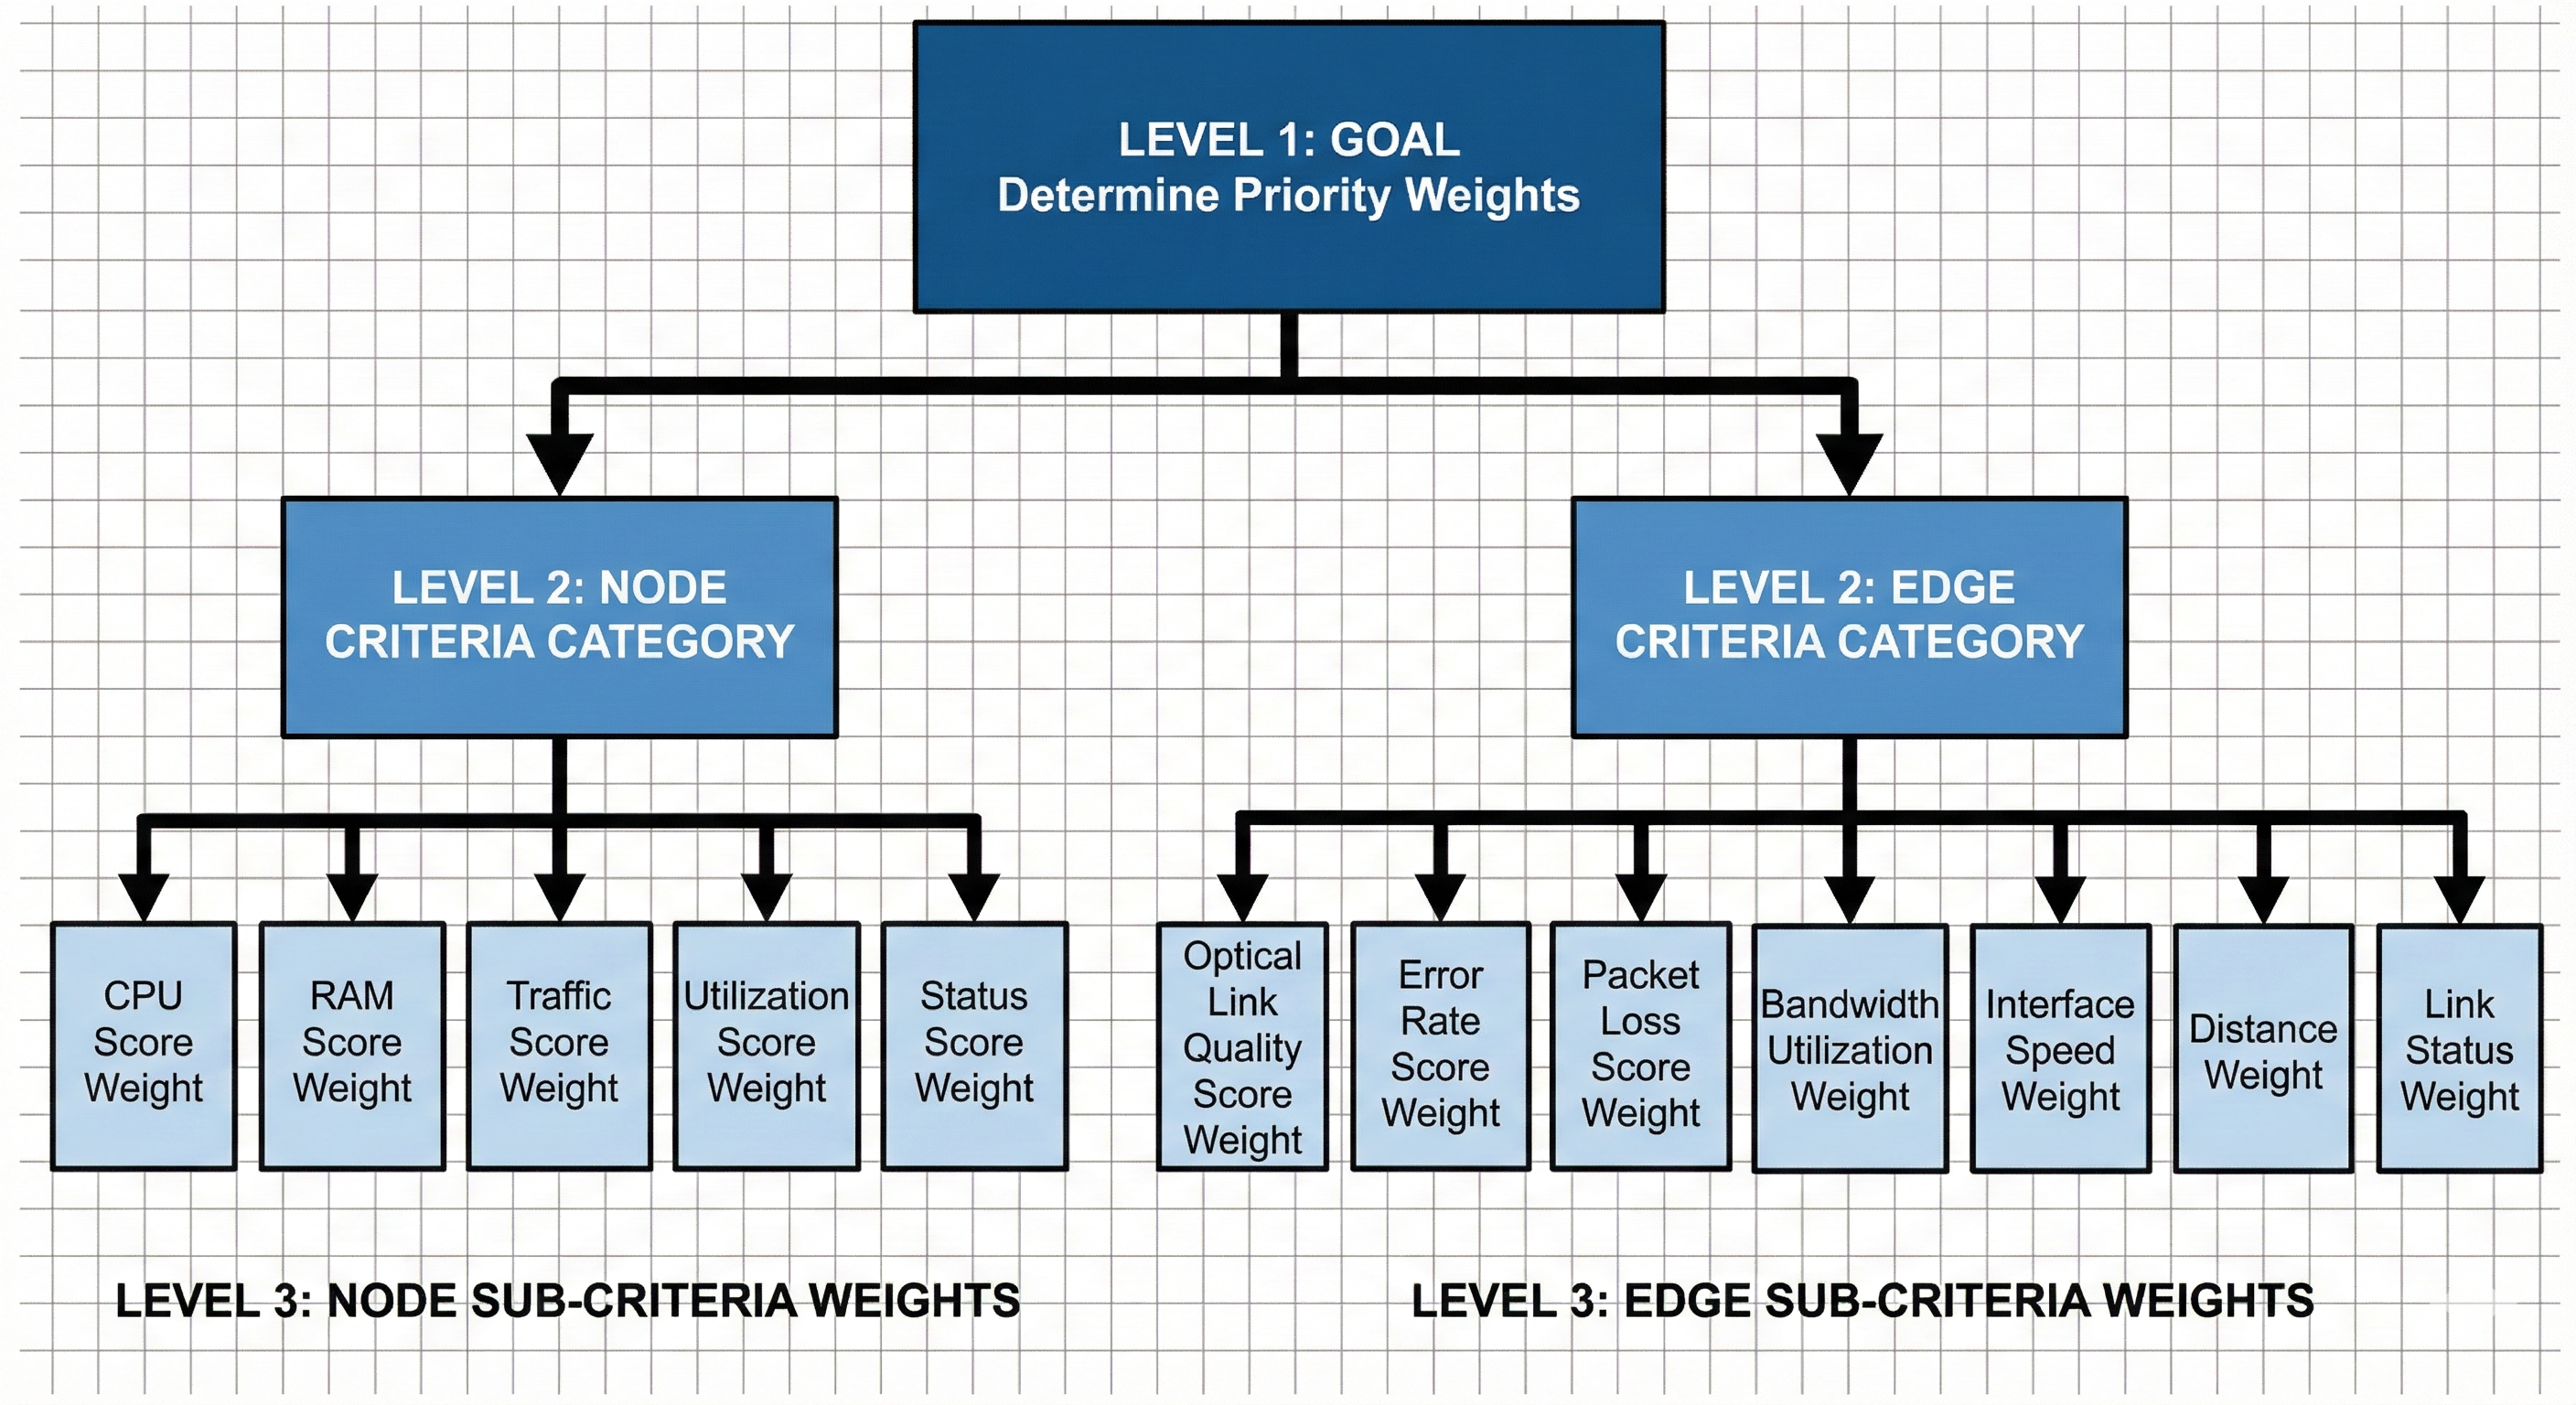
\includegraphics[width=0.9\textwidth]{images/hirarki.png}
    \caption{Struktur Hierarki AHP untuk Penentuan Bobot Parameter}
    \label{fig:ahp_hierarchy}
\end{figure}

\subsubsection{Tahapan Metode AHP}

Implementasi AHP dalam penelitian ini mengikuti lima tahapan sistematis yang dijelaskan sebagai berikut:

\paragraph{1. Penyusunan Matriks Perbandingan Berpasangan}

Tahap pertama adalah membuat matriks perbandingan berpasangan untuk kriteria-kriteria yang telah ditentukan. Setiap pasangan kriteria dibandingkan untuk menentukan tingkat kepentingan relatifnya berdasarkan skala Saaty 1-9.

Matriks perbandingan berpasangan dapat dinyatakan sebagai:

\begin{equation}
    \mathbf{A} = \begin{bmatrix}
        1 & a_{12} & a_{13} & \cdots & a_{1n} \\
        1/a_{12} & 1 & a_{23} & \cdots & a_{2n} \\
        1/a_{13} & 1/a_{23} & 1 & \cdots & a_{3n} \\
        \vdots & \vdots & \vdots & \ddots & \vdots \\
        1/a_{1n} & 1/a_{2n} & 1/a_{3n} & \cdots & 1
    \end{bmatrix}
\end{equation}

\noindent dimana $a_{ij}$ merepresentasikan tingkat kepentingan kriteria $i$ terhadap kriteria $j$. Matriks ini bersifat resiprokal, yang berarti:

\begin{equation}
    a_{ji} = \frac{1}{a_{ij}}
\end{equation}

Sebagai contoh, jika optical link quality dinilai 3 kali lebih penting dari distance, maka:

\begin{equation}
    a_{optical,distance} = 3 \quad \text{dan} \quad a_{distance,optical} = \frac{1}{3}
\end{equation}

Skala perbandingan yang digunakan mengikuti standar Saaty seperti ditunjukkan pada Tabel \ref{tab:saaty_scale}.

\begin{table}[H]
\centering
\caption{Skala Perbandingan Berpasangan Saaty}
\label{tab:saaty_scale}
\begin{tabular}{|c|l|}
\hline
\textbf{Nilai} & \textbf{Interpretasi} \\
\hline
1 & Kedua elemen sama pentingnya \\
3 & Elemen pertama sedikit lebih penting dari elemen kedua \\
5 & Elemen pertama lebih penting dari elemen kedua \\
7 & Elemen pertama sangat lebih penting dari elemen kedua \\
9 & Elemen pertama mutlak lebih penting dari elemen kedua \\
2, 4, 6, 8 & Nilai antara untuk penilaian yang bersifat kompromistis \\
\hline
\end{tabular}
\end{table}

\paragraph{2. Normalisasi Matriks Perbandingan}

Setelah matriks perbandingan disusun, langkah selanjutnya adalah melakukan normalisasi. Pertama, hitung total nilai setiap kolom:

\begin{equation}
    T_j = \sum_{i=1}^{n} a_{ij}
\end{equation}

Kemudian, setiap elemen matriks dibagi dengan total kolomnya untuk mendapatkan matriks ternormalisasi:

\begin{equation}
    n_{ij} = \frac{a_{ij}}{T_j}
\end{equation}

\noindent dimana $n_{ij}$ adalah elemen ternormalisasi pada baris $i$ dan kolom $j$.

\paragraph{3. Perhitungan Vektor Prioritas dan Bobot}

Dari matriks ternormalisasi, vektor prioritas (\textit{Priority Vector}, PV) dihitung dengan menjumlahkan nilai-nilai dalam setiap baris:

\begin{equation}
    PV_i = \sum_{j=1}^{n} n_{ij}
\end{equation}

Selanjutnya, bobot akhir setiap kriteria diperoleh dengan menormalisasi vektor prioritas:

\begin{equation}
    w_i = \frac{PV_i}{n}
\end{equation}

\noindent dimana $n$ adalah jumlah total kriteria yang dibandingkan. Bobot $w_i$ merepresentasikan tingkat kepentingan relatif dari kriteria $i$ terhadap keseluruhan kriteria, dan memenuhi kondisi:

\begin{equation}
    \sum_{i=1}^{n} w_i = 1
\end{equation}

\paragraph{4. Uji Konsistensi}

Untuk memastikan bahwa perbandingan yang dilakukan konsisten dan dapat diandalkan, AHP menggunakan pengujian konsistensi. Pertama, hitung nilai eigen maksimum:

\begin{equation}
    \lambda_{max} = \sum_{i=1}^{n} T_i \cdot w_i
\end{equation}

Kemudian, hitung \textit{Consistency Index} (CI):

\begin{equation}
    CI = \frac{\lambda_{max} - n}{n - 1}
\end{equation}

Selanjutnya, hitung \textit{Consistency Ratio} (CR) dengan membandingkan CI terhadap \textit{Random Consistency Index} (RI):

\begin{equation}
    CR = \frac{CI}{RI}
\end{equation}

Nilai RI bergantung pada jumlah kriteria yang dibandingkan, seperti ditunjukkan pada Tabel \ref{tab:random_index}.

\begin{table}[H]
\centering
\caption{Nilai Random Consistency Index (RI)}
\label{tab:random_index}
\begin{tabular}{|c|c|c|c|c|c|c|c|c|c|}
\hline
\textbf{n} & 1 & 2 & 3 & 4 & 5 & 6 & 7 & 8 & 9 \\
\hline
\textbf{RI} & 0 & 0 & 0.58 & 0.90 & 1.12 & 1.24 & 1.32 & 1.41 & 1.45 \\
\hline
\end{tabular}
\end{table}

Matriks perbandingan dinyatakan konsisten jika:

\begin{equation}
    CR \leq 0.1
\end{equation}

Jika $CR > 0.1$, maka penilaian perbandingan perlu direvisi karena mengandung inkonsistensi yang signifikan.

\subsubsection{Integrasi AHP dengan GAT}

Dalam penelitian ini, AHP diintegrasikan dengan GAT untuk menghasilkan sistem Traffic Engineering yang cerdas dan selaras dengan kebijakan operasional. Skor yang dihasilkan oleh AHP digunakan sebagai label target dalam proses pelatihan model GAT.

Secara matematis, skor kualitas jalur dapat diformulasikan sebagai:

\begin{equation}
    Q_{path} = \sum_{i=1}^{n_{node}} w_i^{node} \cdot f_i(\text{node}) + \sum_{j=1}^{n_{edge}} w_j^{edge} \cdot g_j(\text{edge})
\end{equation}

\noindent\textbf{Keterangan:}
\begin{itemize}
    \item $Q_{path}$ : Skor kualitas total sebuah jalur (semakin tinggi semakin baik)
    \item $w_i^{node}$ : Bobot prioritas untuk parameter node ke-$i$ (hasil perhitungan AHP)
    \item $w_j^{edge}$ : Bobot prioritas untuk parameter edge ke-$j$ (hasil perhitungan AHP)
    \item $f_i(\text{node})$ : Nilai atribut perangkat ke-$i$ (misalnya: sisa kapasitas CPU dalam \%)
    \item $g_j(\text{edge})$ : Nilai atribut koneksi ke-$j$ (misalnya: optical signal quality atau bandwidth tersedia)
    \item $n_{node}$ : Jumlah parameter node yang dipertimbangkan (dalam penelitian ini: 5 kriteria)
    \item $n_{edge}$ : Jumlah parameter edge yang dipertimbangkan (dalam penelitian ini: 7 kriteria)
\end{itemize}

Formula agregasi ini mengadopsi pendekatan weighted composite scoring yang umum digunakan dalam multi-criteria decision making untuk network path selection \cite{weighted_composite_routing, qos_composite_metric, madm_heuristic_routing}. Setiap komponen dinormalisasi dan dikalikan dengan bobot yang ditentukan melalui AHP, menghasilkan skor holistik yang mencerminkan kualitas keseluruhan node dan edge \cite{routing_multiple_optimality, rpso_link_quality}.

Alur kerja integrasi AHP-GAT dapat dijelaskan sebagai berikut:

\begin{enumerate}
    \item \textbf{Tahap Pra-komputasi AHP}: Administrator jaringan atau pakar melakukan penilaian perbandingan berpasangan untuk menentukan tingkat kepentingan relatif dari setiap parameter jaringan (CPU, RAM, optical quality, error rate, bandwidth, dll.). Hasil perhitungan AHP menghasilkan vektor bobot $\mathbf{w}$.

    \item \textbf{Pemberian Label}: Untuk setiap jalur yang mungkin dalam topologi jaringan, skor kualitas $Q_{path}$ dihitung menggunakan formula di atas berdasarkan kondisi jaringan aktual dan bobot AHP. Skor ini menjadi ground truth label untuk pelatihan.

    \item \textbf{Pelatihan GAT}: Model GAT dilatih untuk memprediksi skor kualitas jalur berdasarkan fitur-fitur node dan edge. Fungsi loss yang digunakan adalah:
    \begin{equation}
        \mathcal{L} = \frac{1}{N_{paths}} \sum_{p=1}^{N_{paths}} (Q_{path}^{pred} - Q_{path}^{AHP})^2
    \end{equation}
    dimana $Q_{path}^{pred}$ adalah prediksi model GAT dan $Q_{path}^{AHP}$ adalah label dari perhitungan AHP.

    \item \textbf{Inferensi Real-time}: Setelah model terlatih, GAT dapat memprediksi kualitas jalur secara real-time tanpa perlu menghitung ulang bobot AHP, karena pengetahuan pakar telah terinternalisasi dalam parameter model.
\end{enumerate}

\section{Penelitian Terkait}

Tinjauan studi dilakukan untuk memetakan posisi penelitian ini terhadap penelitian-penelitian sebelumnya yang relevan (\textit{State of the Art}). Pemetaan ini bertujuan untuk mengidentifikasi kesenjangan penelitian (\textit{research gap}) dan memastikan kebaruan kontribusi yang ditawarkan.

Penelitian pertama oleh Marouani dkk. (2024) menerapkan \textit{Graph Attention Networks} (GAT) untuk \textit{Traffic Engineering} pada jaringan WAN. Penelitian tersebut membuktikan bahwa mekanisme \textit{attention} pada GAT mampu menangani topologi dinamis lebih baik daripada metode heuristik konvensional \cite{marouani2024}. Namun, penelitian ini hanya berfokus pada metrik performa teknis murni tanpa mempertimbangkan preferensi kebijakan manajemen jaringan yang seringkali bersifat subjektif pada ISP lokal.

Penelitian kedua oleh Almasan dkk. (2022) mengusulkan pendekatan \textit{Deep Reinforcement Learning} (DRL) yang digabungkan dengan GNN untuk optimasi \textit{routing}. Hasilnya menunjukkan kemampuan generalisasi yang kuat terhadap topologi baru \cite{almasan2022}. Meskipun efektif, pendekatan DRL memerlukan lingkungan simulasi yang sangat kompleks dan waktu pelatihan yang lama, yang menjadi kendala jika diterapkan pada infrastruktur ISP skala menengah dengan sumber daya terbatas.

Penelitian ketiga oleh Rahman dan Hasan (2023) menggunakan \textit{Graph Convolutional Network} (GCN) untuk memprediksi aliran trafik \cite{rahman2023}. GCN efektif dalam menangkap fitur spasial, namun memiliki keterbatasan karena memberikan bobot yang seragam pada tetangga \textit{node} (isotropik), sehingga kurang sensitif terhadap variasi kualitas \textit{link} yang signifikan pada jaringan nirkabel atau campuran.

Berdasarkan tinjauan di atas, ditemukan celah permasalahan di mana belum ada penelitian yang menggabungkan kemampuan adaptif GAT dalam mempelajari topologi graf dengan metode pembobotan multikriteria (\textit{Analytic Hierarchy Process} - AHP). Integrasi ini penting untuk memastikan bahwa rekomendasi AI tidak hanya optimal secara matematis, tetapi juga valid menurut standar operasional dan intuisi pakar jaringan (\textit{Network Engineer}). Rangkuman perbandingan penelitian ditunjukkan pada Tabel \ref{tab:state_of_the_art}.

\begin{table}[ht]
    \centering
    \caption{State of the Art Penelitian}
    \label{tab:state_of_the_art}
    \small
    \begin{tabular}{p{3cm} p{3cm} p{2.5cm} p{4.5cm}}
        \hline
        \textbf{Peneliti (Tahun)} & \textbf{Masalah} & \textbf{Metode} & \textbf{Hasil \& Perbedaan} \\
        \hline
        \cite{marouani2024} & Optimasi trafik pada WAN & GAT & Unggul di topologi dinamis. \textbf{Bedanya:} Penelitian ini menambahkan validasi pakar via AHP. \\
        \hline
       \cite{almasan2022} & Optimasi \textit{Routing} & DRL + GNN & Generalisasi baik tapi training berat. \textbf{Bedanya:} Penelitian ini menggunakan \textit{Supervised Learning} yang lebih efisien. \\
        \hline
        \cite{rahman2023} & Prediksi Trafik & GCN & Efektif spasial. \textbf{Bedanya:} GAT memiliki mekanisme \textit{attention} yang lebih presisi dibanding GCN. \\
        \hline
        \textbf{Penelitian Ini} & \textbf{Rekomendasi Jalur ISP} & \textbf{GAT + AHP} & \textbf{Integrasi \textit{expert judgment} (AHP) ke dalam arsitektur \textit{Deep Learning} (GAT).} \\
        \hline
    \end{tabular}
\end{table}

\section{Kerangka Pemikiran}

Kerangka pemikiran menggambarkan alur logika penelitian dari variabel yang diobservasi hingga pengukuran keberhasilan. Sesuai dengan pendekatan sistem cerdas, kerangka ini disusun dalam empat komponen utama: \textit{Indicators}, \textit{Proposed Method}, \textit{Objectives}, dan \textit{Measurement}.

\begin{enumerate}
    \item \textbf{Indicators (Observed Variables):} Merupakan parameter input yang diambil dari perangkat jaringan, terdiri dari parameter Node (CPU, RAM, Trafik, Utilisasi, Status) dan parameter Edge (Optical Link Quality, Error Rate, Packet Loss, Bandwidth Utilization bidirectional, Interface Speed kedua endpoint, Jarak, Status).

    \item \textbf{Proposed Method:} Solusi yang diusulkan menggabungkan dua metode utama. Pertama, \textit{Analytic Hierarchy Process} (AHP) digunakan pada tahap pra-pemrosesan untuk memberikan bobot prioritas valid berdasarkan penilaian pakar. Kedua, \textit{Graph Attention Network} (GAT) digunakan sebagai algoritma pembelajaran utama untuk mengenali pola topologi dan memprediksi kualitas jalur.

    \item \textbf{Objectives:} Tujuan akhir dari sistem adalah menghasilkan model rekomendasi jalur yang memiliki akurasi tinggi dan mampu mengoptimalkan distribusi trafik jaringan.

    \item \textbf{Measurement:} Keberhasilan metode diukur menggunakan metrik statistik \textit{Root Mean Square Error} (RMSE) untuk performa regresi, dan \textit{Accuracy} untuk mengukur ketepatan klasifikasi kualitas jalur yang direkomendasikan.
\end{enumerate}

Visualisasi kerangka pemikiran penelitian ditunjukkan pada Gambar \ref{fig:kerangka_pemikiran}.

\begin{figure}[ht]
    \centering
    \resizebox{\textwidth}{!}{%
    \begin{tikzpicture}[
        node distance=0.5cm,
        box/.style={draw, rounded corners, minimum width=3cm, minimum height=1cm, align=center, font=\small},
        groupbox/.style={draw, rounded corners, inner sep=0.3cm, align=center},
        arrow/.style={->, thick, >=stealth}
    ]

    % --- COLUMN 1: INDICATORS ---
    \node[font=\bfseries] (ind_title) {INDICATORS};

    \node[box, below=0.5cm of ind_title, fill=white] (cpu) {CPU \& RAM\\Usage};
    \node[box, below=0.3cm of cpu, fill=white] (traf) {Traffic \&\\Utilization};
    \node[box, below=0.3cm of traf, fill=white] (link) {Optical Quality\\Error Rate};
    \node[box, below=0.3cm of link, fill=white] (bw) {Bandwidth\\Availability};
    \node[box, below=0.3cm of bw, fill=white] (dist) {Distance \&\\Status};

    % Frame for Indicators
    \node[groupbox, fit=(cpu)(dist), label=below:\textit{Observed Variables}] (ind_group) {};

    % --- COLUMN 2: PROPOSED METHOD ---
    \node[font=\bfseries, right=1.5cm of ind_title] (met_title) {PROPOSED METHOD};

    \node[box, below=0.5cm of met_title, fill=gray!10, minimum width=4cm] (data) {Dataset Generation\\(Topology \& Metrics)};
    \node[box, below=0.8cm of data, fill=gray!10, minimum width=4cm] (ahp) {\textbf{Weighting Strategy}\\Analytic Hierarchy Process\\(AHP)};
    \node[box, below=0.8cm of ahp, fill=gray!20, minimum width=4cm, minimum height=1.5cm] (gat) {\textbf{Learning Algorithm}\\Graph Attention Network\\(Multi-Head Attention)};
    \node[box, below=0.8cm of gat, fill=gray!10, minimum width=4cm] (pred) {Path Quality\\Predictor};

    \node[groupbox, fit=(data)(pred)] (met_group) {};

    % --- COLUMN 3: OBJECTIVES ---
    \node[font=\bfseries, right=1cm of met_title] (obj_title) {OBJECTIVES};

    \node[circle, draw, align=center, minimum size=2.5cm, below=2cm of obj_title] (obj1) {High Accuracy\\Model};
    \node[circle, draw, align=center, minimum size=2.5cm, below=0.5cm of obj1] (obj2) {Optimal Path\\Recommendation};

    % --- COLUMN 4: MEASUREMENT ---
    \node[font=\bfseries, right=1cm of obj_title] (meas_title) {MEASUREMENT};

    \node[box, below=2cm of meas_title] (rmse) {Root Mean\\Square Error (RMSE)};
    \node[box, below=0.5cm of rmse] (acc) {Model\\Accuracy};
    \node[box, below=0.5cm of acc] (time) {Inference Time};

    \node[groupbox, fit=(rmse)(time), label=below:\textit{Observed Results}] (meas_group) {};

    % --- ARROWS ---
    \draw[arrow, dashed] (ind_group.east) -- (met_group.west);
    \draw[arrow] (data) -- (ahp);
    \draw[arrow] (ahp) -- (gat);
    \draw[arrow] (gat) -- (pred);
    \draw[arrow] (met_group.east) -- (obj1.west);
    \draw[arrow] (met_group.east) -- (obj2.west);
    \draw[arrow] (obj1.east) -- (rmse.west);
    \draw[arrow] (obj1.east) -- (acc.west);
    \draw[arrow] (obj2.east) -- (time.west);

    \end{tikzpicture}%
    }
    \caption{Kerangka Pemikiran GAT berbasis AHP}
    \label{fig:kerangka_pemikiran}
\end{figure}
